% !TEX root = ../main.tex
\chapter{Model creation} \label{ch:model}
% TITOLO DA VALUTARE

This chapter will outline the approach suggested by IBM Reserch for tackling the challange introduced in \textbf{\nameref{ch:introduction}} regarding fault detection and diagnosis (FDD). %TODO

\section{State of the art}
Nowadays, as extensively analyzed by \textcite{methods_for_diagnostic}, FDD approaches fall in either one of the following three categories: physycal model based approaches, data driven approaches and rule-based approaches. The rationales behind these approaches are detailed in \autoref{subsec:phy_models}, \autoref{subsec:data_models} and in \autoref{subsec:rule_models}. Still, each of these approaches share common limitations that can be summarized as
\begin{itemize}
  \item they can be applied to a single, specific building
  \item they requires large manual effort and expertise
  \item deploy can take several weeks
  \item they neglect strong interactions between systems
\end{itemize}

\subsection{Physycal model approach} \label{subsec:phy_models}
These approaches require a physycal model (e.g ordinary differential equations) of the building and its components. They are highly precise in diagnosing faults given a correct model, however, deriving the models is no trivial task and requires times and expertise. On top of this, derived models are building, system and location specific and are difficult to adapt to other buildings than the one they are thought for even if they share similar structure and similar components, thus limiting the scalability of this approach.

\subsection{Data driven approach} \label{subsec:data_models}
Data driven approaches completely rely on building's sensor data. They assume that access to a large dataset of hystorical data is granted. There's little to no need for any \textit{a priori} knowledge of the processes involved. Black-box data driven approaches derive the model in the form of a input-output relationship which parameters aren't correlated with the actual physical parameter (e.g artificial neural networks, regression) while grey-box data driven approaches take advantage of simplified physical relationships between measured quantities (e.g principal component analysys) and rely on statistical methods for estimating their parameters. Even though these methods don't suffer from scalability issues they are limited to fault detection and lack in diagnosis capabilities.

\subsection{Rule-based approach} \label{subsec:rule_models}
The rule-based approach is the most common in traditional FDD applications. It uses domain knowledge and expertise in order to derive a series of simple \textit{if-then-else} rules or some kind of decision trees along with a series of thresholds and confidence intervals; during system operations data are evaluated against this rules and countermeasures are eventually taken. Even though this is the most common approach, it still needs a lot of manual effort and requires access to domain knowledge so these requirements still limit portability and scalability of applications based on this technique.

\section{IBM Research approach}
The approach developed by IBM Research is based on a combination of the three aformentioned concepts to overcome their disadvantages. It models high level physical processes in the systems to derive diagnosis rules, it parametrize the rules using data analytics techniques and applies them during systmes operations. The strength of the semantic approach lies in its capability to automatically infer knowledge given a building, its sensors and their data. This lead to a semi-automated process that limit the manual effort needed, as shown in \autoref{fig:approach_overview}.
\begin{figure}
  \centering
  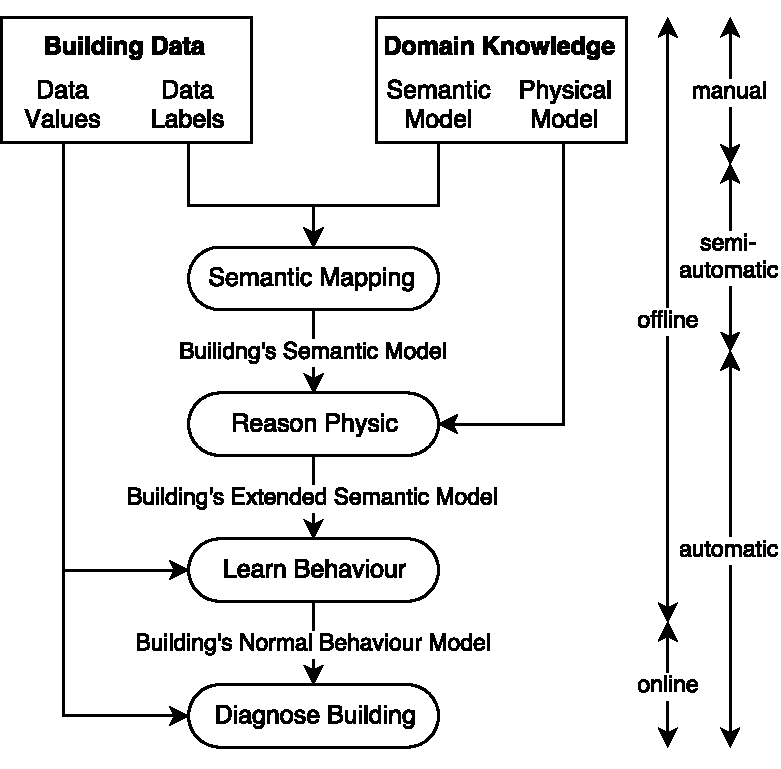
\includegraphics[width=0.7\textwidth]{approach_overview.pdf}
  \caption{IBM Reserch approach, overview}
  \label{fig:approach_overview}
\end{figure}

The proposed approach needs 3 inputs to produce the diagnosis of a given anomaly
\begin{itemize}
  \item building data: assumed available in the building's Building Management System (BMS)
  \item semantic model: specified through the use of concepts from domain ontologies Brick (\autoref{subsec:brick}) e SSNO (\autoref{subsec:ssn})
  \item physycal model: the model of the physical dependencies between subsystems of the building. The physical processes are modelled through concepts presented in the extended SSNO (\autoref{ssubsec:extended_ssno})
\end{itemize}
these inputs are processed through the various stages to produce the complete model of the building and its internal processes. Details about the different phases are given in the following pages.

\subsection{Semantic Mapping} \label{subsec:semantic_mapping}
Building a semantic model for a specific building needs knowledge on the type of sensors, meters and various equipment available in said building, their location and their semantic meaning in the chosen ontologies. These informations are usually stored in BMS through labels that, despite some kind of standardization efforts, are usually vendor specific; in some cases even the same vendor ends up changing its labeling schemes throughout the years. Even though there is no common ground to evaluate these labels, usually they are comprised of a series of abbreviations, eventually separated by some special character (e.g ``\textunderscore''), that gives informations about the device's ID, function and location (or the equipment it is part of). An air temperature sensor in a room on ground floor can be labeled AIR\textunderscore TEMP\textunderscore R3GF while another air temperature sensor in a room on the first floor may ends up being labeled as RATSF1R9; both the sensors represent a common semantic resource in an ontology and need to be mapped that concept. This process is called semantic mapping. Existing approaches are differentiated in three different types \cite{semantic_mapping}
\begin{itemize}
  \item semi-automatic: they offer a tool assisting the user in labelling the point to corresponding semantic types and are based on advanced text mining techniques (e.g regular expressions, classifiers)
  \item data driven: these approaches try to recover the meta-data given the timeseries. It is based on the concept that different data-points exhibiting similar timeseries behaviour should be similar themselves.
  \item active feedback: in these kind of approaches a series of known events are injected into the system and datapoints semantic model is derived observing the effect of the event injection.
\end{itemize}

\subsubsection{Building Energy Asset Discovery tool}
BEAD \cite{bead} is the tool developed by IBM Research for assisting user in the process of discovery and tagging of sensors. The tool is based on dictionaries of the type $\mathcal{D}:\mathcal{A}\rightarrow \mathcal{MS}$ where $\mathcal{A}$ is the set of all relevant acronyms and $\mathcal{MS}$ is the set of markerset; each markerset is a set of markers, or keywords. These concepts are closely related to those of tagset and tag found in the Brick ontology and this duality allows the association of the sensor with the correct semantic type as described by Brick (see \ref{subsec:brick}). The dictionary contains the most common acronyms found in BMS and it is further extended by the markers (tags) from the Brick ontology, such that a tag maps to itself, e.g Temperature$\rightarrow$\{Temperature\}. The tool take a label from the BMS and compute a similarity score against the dictionary entries and guide the user in the labeling process. For example, given the following dictionary
\begin{description}[noitemsep]
  \item \textbf{d1}: RAT$\rightarrow$\{Return, Air, Temperature\}
  \item \textbf{d2}: RAT$\rightarrow$\{Room, Air, Temperature\}
  \item \textbf{d3}: SAT$\rightarrow$\{Supply, Air, Temperature\}
  \item \textbf{d4}: OAT$\rightarrow$\{Outdoor, Air, Temperature\}
  \item \textbf{d5}: Temp$\rightarrow$\{Temperature\}
  \item \textbf{d6}: Temperature$\rightarrow$\{Temperature\}
\end{description}
the label RATSF1R9 (Room Air Temperature Sensor, Floor 1, Room 9) has a high similarity with both RAT$\rightarrow$\{Return, Air, Temperature\} and RAT$\rightarrow$\{Room, Air, Temperature\}, so it's up to the user to understand the meaning and choose the right markerset. In a similar fashion it is possible to extract information on the location of a sensor or the asset it is related to, as shown in \autoref{tab:bead_dictionary}.
\begin{table}
  \centering
  \caption{Dictionary extended with assets' informations}
  \label{tab:bead_dictionary}
  \begin{tabular}{lll}
    \hline
    \textbf{Label} & \textbf{Asset} & \textbf{Marketset}                       \\\cline{1-3}
    U6\textunderscore RAT        & AHU6  & \{Return, Air, Temperature\}    \\
    U6\textunderscore DAT        & AHU6  & \{Discharge, Air, Temperature\} \\
    AHU7\textunderscore RAT      & AHU7  & \{Return, Air, Temperature\}    \\
    AHU7\textunderscore SAT      & AHU7  & \{Supply, Air, Temperature\}    \\
    AU9\textunderscore RET\textunderscore TEMP & AHU9  & \{Return, Air, Temperature\}    \\
    AU9\textunderscore SUP\textunderscore TEMP & AHU9  & \{Supply, Air, Temperature\}
  \end{tabular}
\end{table}

this process clearly requires human supervision, hence the definition of semi-automatic, but through this approach the operator has to manually inspect a smaller subset of all the possible marketsets \cite{semantic_mapping} thus taking minutes instead of several weeks to complete the semantic mapping. The output of this process is the semantic model of the specific building according to the chosen ontology. A chart illustrating the whole process is shown in \autoref{fig:semantic_mapping}.

\begin{figure}
  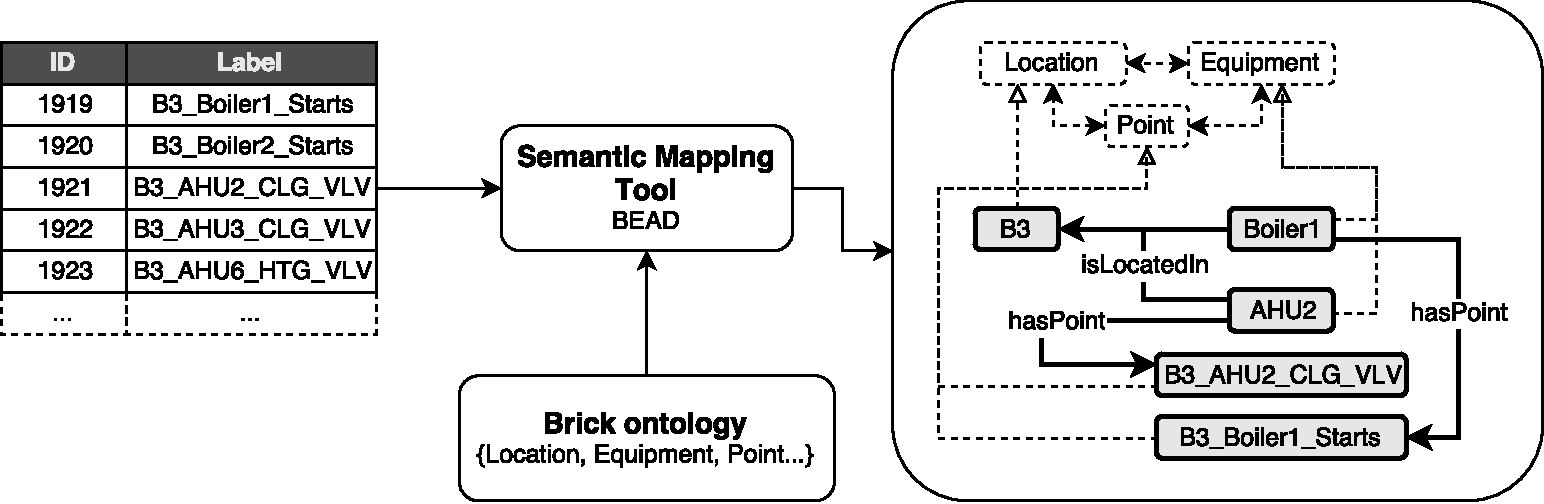
\includegraphics[width=1\textwidth]{semantic_mapping.pdf}
  \caption{Semantic mapping process}
  \label{fig:semantic_mapping}
\end{figure}

\section{Physic model inference}
The semantic model obtained from the semantic mapping phase is a model of the building architecture, assets, sensors and their loaction across the building. The model still lacks information about the physic processes taking place in the building and how the actual physic model is monitored and influenced by the points (sensors, setpoints etc.) in the building. Manually building the physical model of a building is unpractical and costly, thus the developed framework approaches this challange through the use of semantic inference techniques. This phase requires as inputs the semantic model of the building and an appropriate ontology that models the physics variables. % TODO something about difference between modelling the upper ontology and creating the actual model
Given those inputs, through the reasoning process is possible to automatically add the correct dependencies and physical processes to the model. This process is separated in two phases:
\begin{itemize}
  \item physical properties inference: it recreates the physical variables that are involved in physical processes. The properties are either mandatory or optional.
  \item physical processes inference: once the physical properties are set in place, it is possible to link them together according to the domain knowledge specified in the upper ontology.
\end{itemize}

\subsection{Physical properties inference}
Properties represent physical quantities in the real world and can be mandatory or optional. Mandatory property are characteristic of a ssn:FeatureOfInterest and need to be created for each instance of that feature. For example, in \autoref{fig:mandatory_properties} it is shown that the concept of :Room phy:requiresProperty :Temperature, that means that every instance of a :Room needs to be associated with a property that is an instance of :Temperature, or in plain english that every room has a temperature, therefore :Temperature is a mandatory property.
\begin{figure}
  \centering
  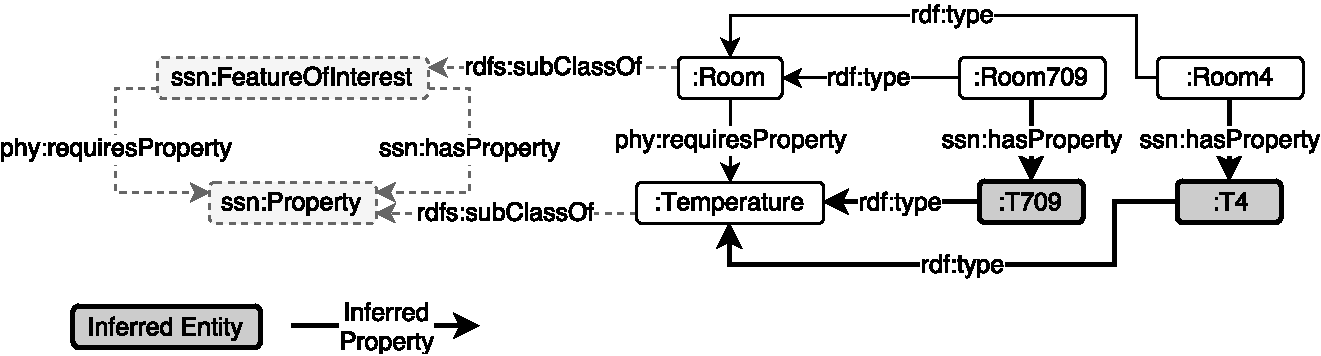
\includegraphics[width=1\textwidth]{reason_mandatory.pdf}
  \caption{Process of inference of mandatory properties.}
  \label{fig:mandatory_properties}
\end{figure}
Optional properties, on the other hand, need to be created only if some requirements are met, for example a :Room have a :Cooling property only if a :CoolingActuator is present in said room, and it is modeled in the upper ontology as :CoolingActuator phy:defaultObserved :Cooling.

\subsection{Physical processes inference}
Once all the actual properties have been infered for a specific configuration, it is time to append to the model informations about the physical processes involving such properties. As already stated in \autoref{ssubsec:extended_ssno}, physical processes are modeled as Linear Time Invariant (LTI) systems based on the fact that Multiple Input Multiple Output (MIMO) processes can be decomposed into multiple Multiple Input Multiple Output (MISO) processes. A MISO process can be further subclassed as a Single Input Single Output process. Each process follows the rules
\begin{description}[noitemsep]
  \item\textbf{Rule 1} a process has at least one input and exactly one output
  \item\textbf{Rule 2} when a process has multiple inputs, they superpose additively
\end{description}
given these rules, it is possible to define a class hierarchy of LTI processes that are used to model a physical system. A subset of said taxonomy is available at \autoref{tab:lti_taxonomy}.
\begin{table}
  \centering
  \caption{Taxonomy of the semantic representation of LTI processes}
  \label{tab:lti_taxonomy}

  \begin{tabular}{lll}\hline
    \textbf{Semantic concept} & \textbf{Parent} & \textbf{Formal definition} \\\hline
    MISO & Process & $y_i(t)=\mathbf{c_i}\cdot \mathbf{x_i}+\mathbf{d_i}\cdot \mathbf{u_i}(t)=f(\mathbf{u}(t))$ \\\hline
    SISO & MISO & $y_i(t)=\mathbf{c_i}\cdot \mathbf{x_i}+d_i\cdot u_i(t)=f(u(t))$ \\\hline
    Positive Correlted (PC) & SISO & $y(t)\propto u(t)$ \\
    Negative Correlated (NC) & SISO & $y(t)\propto -u(t)$ \\
    Proportional (P) & SISO & $y(t)=k_p\cdot u(t)$ \\
    Positive Proportional (PP) & PC, P & $y(t)=k_p\cdot u(t), k_p\geq 0$\\
    Negative Proportional (NP) & NC, P & $y(t)=k_p\cdot u(t), k_p<0$\\
    Negation (N) & NP & $y(t)=k_p\cdot u(t), k_p=-1$\\
    Integral (I) & P & $y(t)=k_I\int u(t)dt$\\
    Derivative (D) & P & $y(t)=k_D\cdot\dot u(t)$\\
    Lag (PTn) & P & $\sum_{i=0}^{n}C_i\cdot T^i \cdot y^{(i)}(t)=k_{PT}\cdot u(t) $\\
    1\textsuperscript{st} order lag (PT1) & PTn & $T\cdot\dot y(t)+y(t)=k_{PT}\cdot u(t)$\\
    Delay ($\tau$) & SISO & $y(t)=u(t-\tau), \tau>0$\\
    Multiplicative (M) & MISO & $y(t)=u_1(t)\cdot u_2(t)$
  \end{tabular}
\end{table}

\subsection{Example of the reasoning process}
In order to better explain the concepts presented in the previous sections an example of the full process applied to a room, facing the outside environment, with a cooling Air Handling Unit (AHU). At the end of the section it is shown that a full model of the room, its internal and external processes is derived. This model will then be used during the explanation of the diagnosis process. Looking back at \autoref{fig:approach_overview}, we start by defining the inputs needed for the process (sharp top boxes).
\paragraph{Building data and semantic model}
It is assumed that some kind of BMS is available in the building so that through the BMS is it possible to retrieve both labels (for semantic mapping) and data of various sensors (useful for diagnosis purposes, see ). % TODO see later chapters
The room analyzed in the example will be named ROOM1. In ROOM1 an air temperature sensor and an occupancy sensor are available. Room1 is also equipped with an AHU, named AHU709 which internal components are observed by a fan mode sensor, a supply air flow sensor,  coil water temperature sensor and a coil water flow sensor. This AHU709 is fed by a chiller named C1 equipped with a power sensor. Let the BMS contains the data as in \autoref{tab:bms_example} and let use Brick (\ref{subsec:brick}) as a domain ontology.
\begin{table}
  \centering
  \caption{Example of BMS content}
  \label{tab:bms_example}
  \begin{tabular}{l|l}
    \hline
    \textbf{ID} & \textbf{Label} \\\hline\hline
    1234 & CCPC1B3 \\\hline
    1235 & CWFU709 \\\hline
    1236 & CWTU709 \\\hline
    1237 & SAFAHU709C1 \\\hline
    1238 & FMAHU709 \\\hline
    1239 & OCCR1 \\\hline
    1240 & ATSROOM1 \\\hline
    1241 & ATS\textunderscore Outside \\\hline
  \end{tabular}
\end{table}
through the semantic mapping tool (\ref{subsec:semantic_mapping}) it is possible to map the labels in the BMS to the Semantic type in the brick ontology. The user can also give the systems additional information about the architecture of the building and the location of equipments and sensors. It is then possible to map :B3 as a brick:Location, :ROOM1 still as brick:Location, and then link one to the other as :ROOM1 brick:isPartOf :B3 and so on. The tool will also discover the semantic type of the sensor and will be able to create the correct instances, for example it will add to the model an air temperature sensor named :ATSROOM1 and will link it as a point to :ROOM1. The output semantic graph can be seen in \autoref{fig:semantic_mapping_example} where the instances created from the BMS and their mutual relationships are bold, while the brick ontology concepts and relationships are light grey.

\begin{figure}
  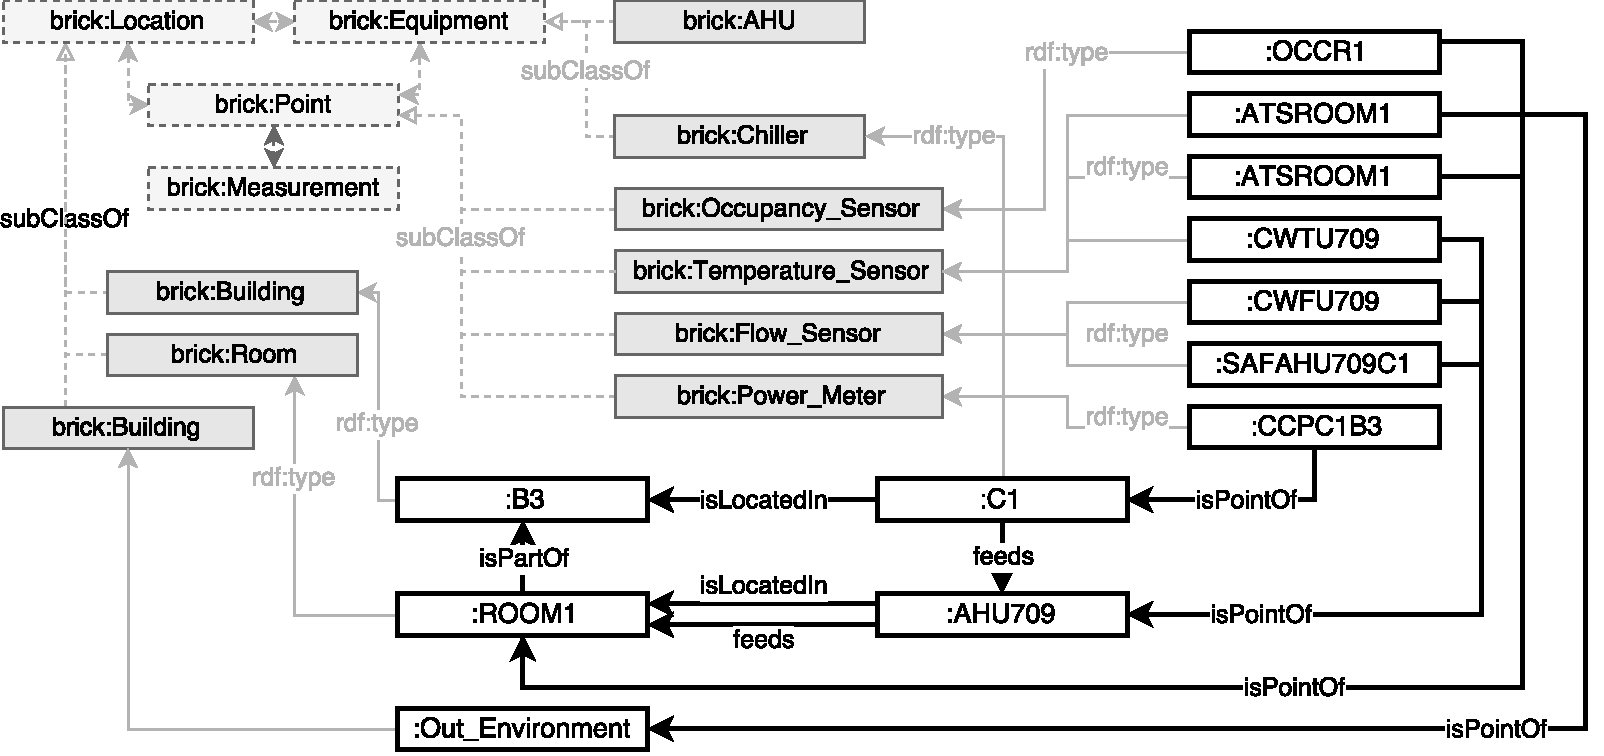
\includegraphics[width=1\textwidth]{semantic_mapping_example.pdf}
  \caption{Complete model for a room in a building equipped with an AHU}
  \label{fig:semantic_mapping_example}
\end{figure}

\paragraph{Physic model}
The physic model is a model of the physic phenomena occuring in an enviroment. It defines physical variable and processes and their interaction in the context of a specific domain. Creating a model of physic laws is a time consuming task that involve expertise from different fields, from engineering to physics, that are very domain specific. The good side of the semantic approach is that once the model is derived from a general point of view, it is automatically extended for every instance of a building, indipendently from its architecture. It is to note that the domain model for the physic does not necessarily model exact physical relationship but just the principal ones, since those are the most relevant to the approach, however this choice is purely paractical rather then a limitation of the approach itself and given sufficient time and knowledge it is possible to enrich the model in order to close the gap with the reality. Here will be presented a model for the physic of a room, equipped with a AHU fed by a chiller. The model is based on a simplification based on the assumption of fully mixed air, that allows for the modeling of a whole space as a single node with uniform temperature. \textcite{building_room_physics} provide an insight of the physic involved in the example. It starts describing a heat balance equation of a room as
\begin{gather}
  m_rc_p\dot{\vartheta_{r}}=Q_{Energy}\label{eq:room_variables}\\
  Q_{Energy}=Q_{Occ}+Q_{Cool}+\sum{A_ih_i(\vartheta_{i}-\vartheta_{r})}\label{eq:energy_composition}\\
\end{gather}

and from \autoref{eq:room_variables} and \autoref{eq:energy_composition}
\begin{equation}
  m_rc_p\dot{\vartheta_{r}}+\sum{A_ih_i\vartheta_{r}}=Q_{Occ}+Q_{Cool}+\sum{A_ih_i\vartheta_{i}} \label{eq:room_lag}
\end{equation}

that says that the temperature of a room $\vartheta_r$ is a first order derivative of the room's inner energy $Q_{Energy}$ that is the combination of the heat gain of occupants $Q_{Occ}$, the heat removed by the cooling system $Q_{Cool}$ and the heat transfer between adjacent environments. Given this equations semantic informations can be extracted.
From \autoref{eq:room_variables} it can be seen that
\begin{enumerate}[noitemsep]
  \item rooms have an internal energy [Property, mandatory]
  \item rooms have a temperature [Property, mandatory]
\end{enumerate}
while from \autoref{eq:energy_composition} it follows that
\begin{enumerate}[noitemsep, resume]
  \item a room's temperature is influenced by the energy in a first order lag process [Process, PT1]
  \item rooms can be cooled and cooling is negative proportional (NP) with the room's energy
  \item room energy depends from the adjacents enviroment's temperature proportional to the shared surface $A_i$ and the heat transfer coefficient $h_i$, hence the dependency is a positive proportional process [Process, PP]
\end{enumerate}
further analyzing the physic involved, bring to the conclusion that
\begin{equation}
  Q_{Occ}=q_{lat}n_{occ} \label{eq:occupancy_heat}
\end{equation}
where $q_{lat}$ is the latent heat gain and $n_{occ}$ the number of occupants in the room. From  \autoref{eq:energy_composition} and \ref{eq:occupancy_heat} it follows that
\begin{enumerate}[noitemsep, resume]
  \item rooms have a number of occupants [Property, Mandatory]
  \item a room's internal energy is positively correlated with the number of occupants [Process, PP]
\end{enumerate}
additional knowledge can be added if the physics of the system in known; for example, it is possible to further enrich the model by specifying the internal processes that regulate a AHU. \textcite{building_ahu_physics} provide a simplified model for modelling the cooling load of an AHU through \autoref{eq:cooling_load}
\begin{equation}
  Q_{Cool}=\frac{c_a\dot{m_{a}^{e}}c_c\dot{m_{c}^{e}}}{c_{a}\dot{m_{a}^{e}}+c_c\dot{m_{c}^{e}}}(\vartheta_{a}-\vartheta_{c}) \label{eq:cooling_load}
\end{equation}
this leads to the following conclusions
\begin{enumerate}[noitemsep, resume]
  \item AHUs are used for cooling [Poperty, mandatory]
  \item cooling is a complex function of the air temperature, the chilled water temperature, the supply air flow and the water flow in the coil [Process, MISO]
\end{enumerate}
\textcite{building_chiller_physics} provide a simple model of a chiller's physic, which equation can be expressed as
\begin{equation}
  \dot{m_c}c_w(\vartheta_{cret}-\vartheta_c)=\eta_{COP}W
\end{equation}
